%\documentclass[12pt]{article}

%\usepackage[italian]{babel}
%\usepackage{listings}
%\usepackage{dcolumn}

%\usepackage{graphicx}
%\begin{document}

%\title{\sc Esercizio 2}

%\maketitle 

\chapter*{Esercizio 2}

%dovrebbe essere un abstract (riassunto) nel relaz_finale
\section*{Scopo dell'esercitazione}
Il programma implementa la struttura di un farm in C-MPI con attribuzione dinamica del carico. Il dominio dei dati in input deve essere partizionato in modo da generare un numero di sottodomini indipendenti (task) che sia maggiore (ad esempio multiplo) rispetto al numero dei processi paralleli (worker) utilizzati.

%non so se dividerlo cosi come si vede nei commenti o meno
\section*{Contenuto del $2^\circ$ esercizio}
Analizziamo come, grazie all'impiego di pi\`u processori su un'architettura distribuita, il tempo di esecuzione di un algoritmo che svolge operazioni aritmetiche viene notevolmente ridotto suddividendo dinamicamente il carico di lavoro.


\section*{Svolgimento}
Segue codice sorgente utilizzato:
\lstinputlisting[language=C, breaklines=true]{farmMOD.c}


\subsection*{Note sul codice}
Descriviamo brevemente come funziona il programma. Vengono impiegati \emph{n} processi paralleli; di questi, quello con \emph{rank = 0} viene chiamato master e i restanti \emph{n-1} processi slave.
Il master inizia per primo a lavorare: inizializza i dati, chiede all'utente il numero di sottodomini da creare ed invia ad ogni slave il primo task.
L'invio di ciascun sottodominio avviene tramite due funzioni \emph{MPI\_Send()}. La prima contiene informazioni circa la dimensione del sottodominio assegnato, la seconda invece invia proprio la porzione di array su cui lo slave dovr\'a operare. Avendo infatti dichiarato come variabile globale l'array data[], ogni processo ne possiede uno; ciascuno slave non fa altro che ricevere parte del vettore appartenente al master per copiarlo all'interno del proprio (inizialmente vuoto).\\
Assegnata a ciascuno slave la porzione di array, il master entra in un loop nel quale attende un risultato da uno slave qualunque (MPI\_ANY\_SOURCE). Allo slave che invia il dato (status.MPI\_SOURCE) il master manda immediatamente il lavoro successivo (selezionato attraverso la funzione \emph{get\_next\_job\_item()}). Al termine dei tasks viene inviato l'avviso di uscita.
Ciascuno slave pu\`o ricevere dal master tre tipi di messaggio: la dimensione dell'array su cui dovr\`a lavorare (identificato dal tag CHUNKTAG), la porzione di array da lavorare (identificato dal tag WORKTAG) oppure il messaggio di fine processo (identificato dal tag DIETAG). I primi due messaggi viaggiano in coppia, l'ultimo invece \`e un messaggio singolo. Lo slave si mette in attesa del primo messaggio, controlla che non sia l'avviso di uscita, qualora non lo fosse si mette nuovamente in attesa per ricevere i dati. Grazie ai tag i processi non rischiano di confondere i messaggi ricevuti.

\subsection*{Analisi delle prestazioni}
Come richiesto dalle consegne abbiamo aggiunto al codice le primitive MPI MPI\_Wtime() per raccogliere informazione sul tempo totale impiegato dal master e quello impiegato da ciascun worker.
I risultati ottenuti compilando e facendo eseguire il codice sono riportati in \emph{Figura \ref{fig:3proc400}}, \emph{Figura \ref{fig:5proc400}} e sono concordi con quanto ci aspettavamo di osservare. 
Variando il numero di processori e dimensione dell'input, i risultati computazionali variano. Ai fini del test, abbiamo mantenuto costante la dimensione del dominio dei dati (160000).

\begin{figure}[htp]
\centering
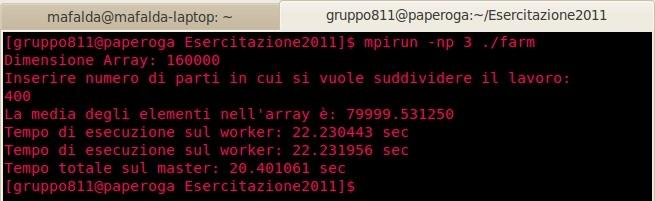
\includegraphics[width=\textwidth]{Immagini_relazione/6_esec3p400.jpeg}
\caption{Utilizzo di 3 processori su 400 sottodomini.}
\label{fig:3proc400}
\end{figure}

\begin{figure}[htp]
\centering
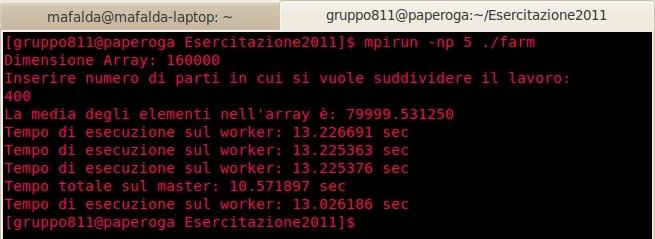
\includegraphics[width=\textwidth]{Immagini_relazione/1_esec5p400.jpeg}
\caption{Utilizzo di 5 processori su 400 sottodomini.}
\label{fig:5proc400}
\end{figure}
\newpage
I risultati mostrano chiaramente come, mantenendo invariato dominio e sottodomini, i tempi di esecuzione dei task variano sensibilmente al variare del numero dei processori impiegati. In \emph{Figura \ref{fig:3proc400}}, a causa dell'impiego di 3 processori, i tempi totali sono quasi raddoppiati rispetto a \emph{Figura \ref{fig:5proc400}}.
\\
\\
A questo punto \`e utile analizzare come varia l'esecuzione del programma al variare del numero di sottodomini. Impieghiamo 5 processi paralleli (come in \emph{Figura \ref{fig:5proc400}}), ma questa volta chiediamo al master di creare 40 sottodomini.


\begin{figure}[htp]
\centering
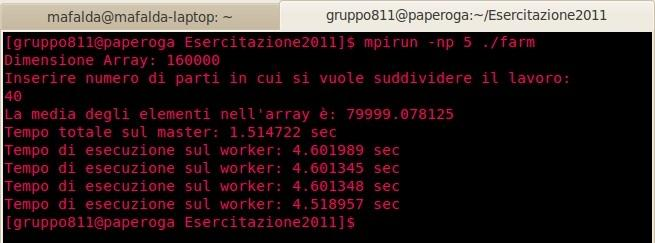
\includegraphics[width=\textwidth]{Immagini_relazione/4_esec5p40.jpeg}
\caption{Utilizzo di 5 processori su 40 sottodomini.}
\label{fig:5proc40}
\end{figure}

Al diminuire del numero di tasks i tempi di esecuzione diminuiscono anch'essi. Possiamo presupporre che questo sia dovuto, specie in questa esercitazione a scopo didattico, della notevole diminuzione del numero di primitive MPI \emph{MPI\_Send()} e \emph{MPI\_Recv()} effettuate da master e slaves per comunicare. Condizione limite \`e che il numero di lavori non sia minore del numero di processori; in tal caso non si apprezzerebbero le potenzialit\`a della struttura a farm.
\\
\newpage
Per un'analisi pi\`u approfondita invece ci viene in aiuto il tool \mbox{\textbf{jumpshot-4}}, che ci consente di visualizzare su un diagramma di Gantt l'andamento dei processi e le loro comunicazioni, secondo la notazione: 

%\begin{center}
\begin{figure}[htp]
\centering
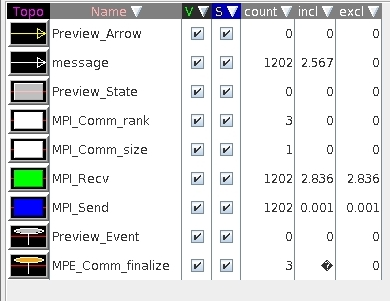
\includegraphics[width=0.53\textwidth]{Immagini_relazione/9_Legenda53pJS.jpg}
\caption{Legenda del tool jumpshot}
\label{}
\end{figure}
%\end{center}


\begin{figure}[htp]
\centering
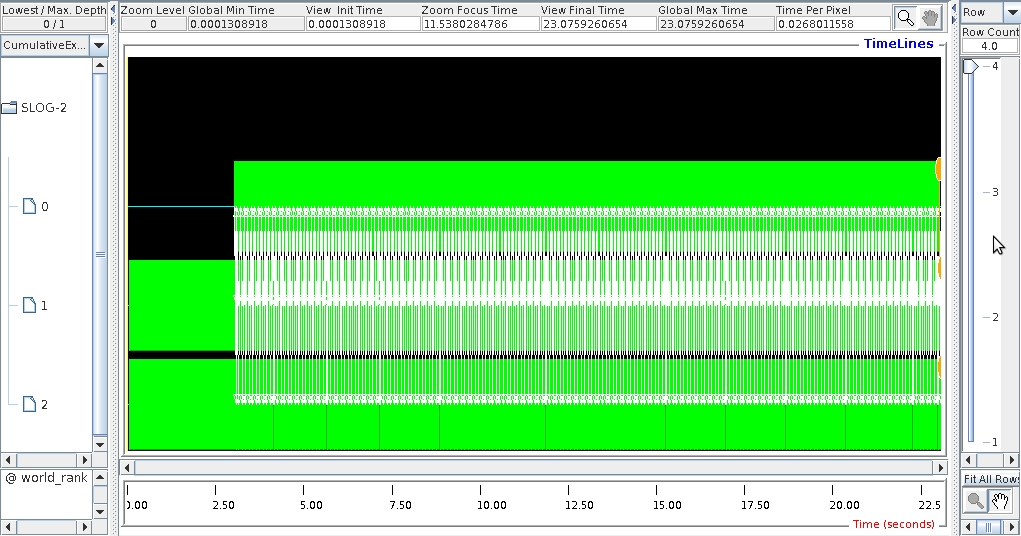
\includegraphics[width=0.83\textwidth]{Immagini_relazione/7_JS3p400.jpg}
\caption{Jumpshot. Utilizzo di 3 processori su 400 sottodomini.}
\label{}
\end{figure}

Queste immagini corrispondono all'esecuzione del codice riporato in \emph{Figura \ref{fig:3proc400}}. Analizzando il grafico mettiamo in evidenza le seguenti cose:
naturalmente i messaggi partono dal master e si susseguono molto ravvicinatamente dal punto di vista temporale. Essendo le comunicazioni molto fitte riportiamo anche uno zoom sull'immagine. (Figura \ref{fig:zoom})
\\
\\
\begin{figure}[htp]
\centering
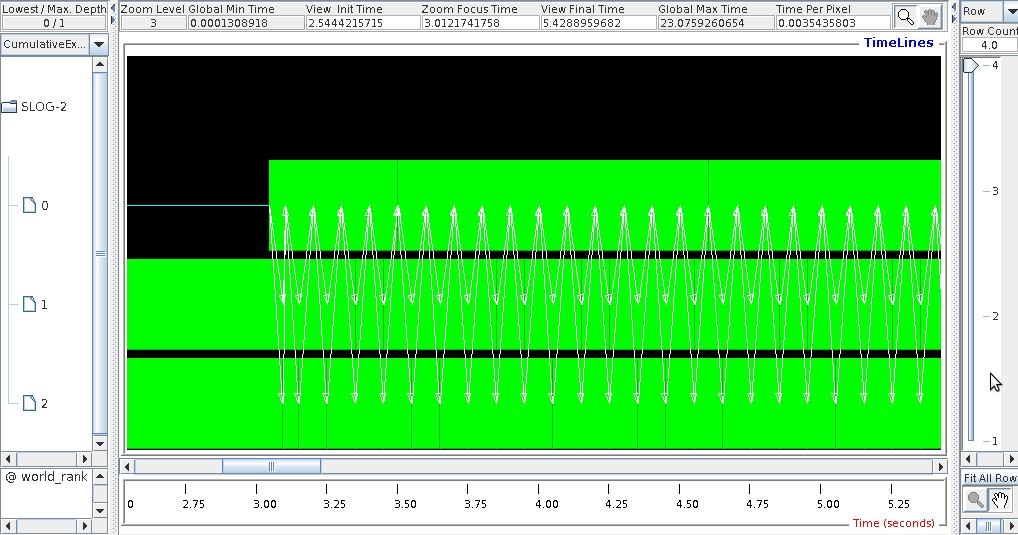
\includegraphics[width=0.84\textwidth]{Immagini_relazione/8_JS3p400Zoom.jpg}
\caption{Jumpshot. Utilizzo di 3 processori su 400 sottodomini. (Zoom)}
\label{fig:zoom}
\end{figure}
\\
Grazie allo Zoom risulta evidente l'interazione tra i processi. Ogni volta che uno slave termina la computazione avvisa il master, che provvede ad inviare il nuovo \emph{work}. Come evidenzia la legenda, l'istante in cui viene effettuata una \emph{MPI\_Send()} \`e colorato di blu (sebbene si veda poco), mentre gli intervalli temporali in cui i processi sono in attesa di \emph{MPI\_Recv()} sono verdi.  
\\
\\
\newpage
Vediamo ora cosa cambia nel diagramma utilizzando 5 processori:
\\

%\begin{frame}

\begin{figure}[htbp]
\centering
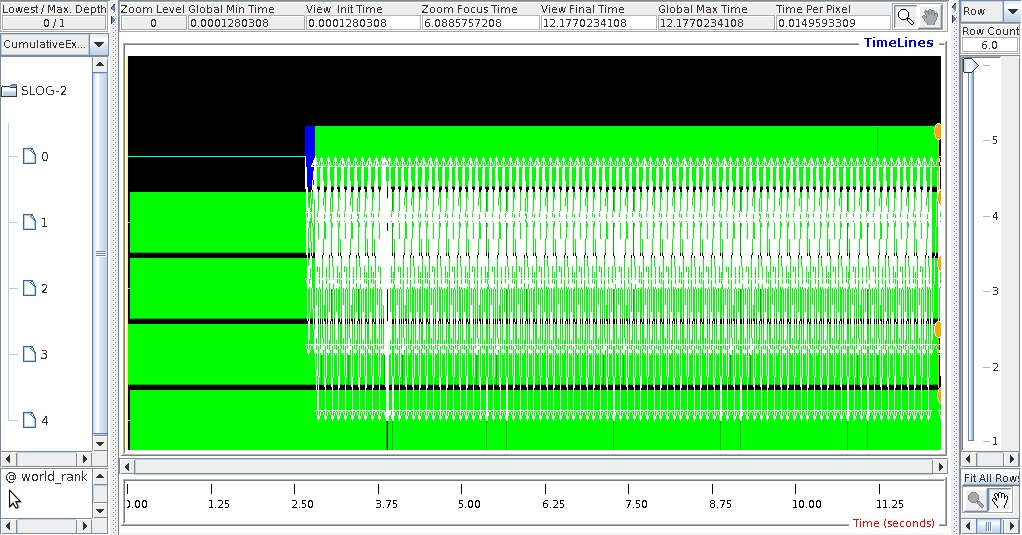
\includegraphics[width=\textwidth]{Immagini_relazione/2_JS5p400.jpg}
\caption{Jumpshot. Utilizzo di 5 processori su 400 sottodomini.}
\label{}
\end{figure}

%\end{frame}

La differenza pi\`u evidente con le immagini precedenti \`e la netta diminuzione del tempo di esecuzione di master e slaves (tempo in ascissa).  \`E interessante notare come all'avvio del processo master, l'intervallo di tempo dedicato alle \emph{MPI\_Send} (zone blu) occupi decisamente pi\`u spazio. Questo momento corrisponde nel codice al \textbf{for} di assegnazione dei primi lavori.
\\
\newpage
Riportiamo ora il risultato fornito da Jumpshot-4 a seguito dell'esecuzione del codice in \emph{Figura \ref{fig:5proc40}}:

\begin{figure}[htbp]
\centering
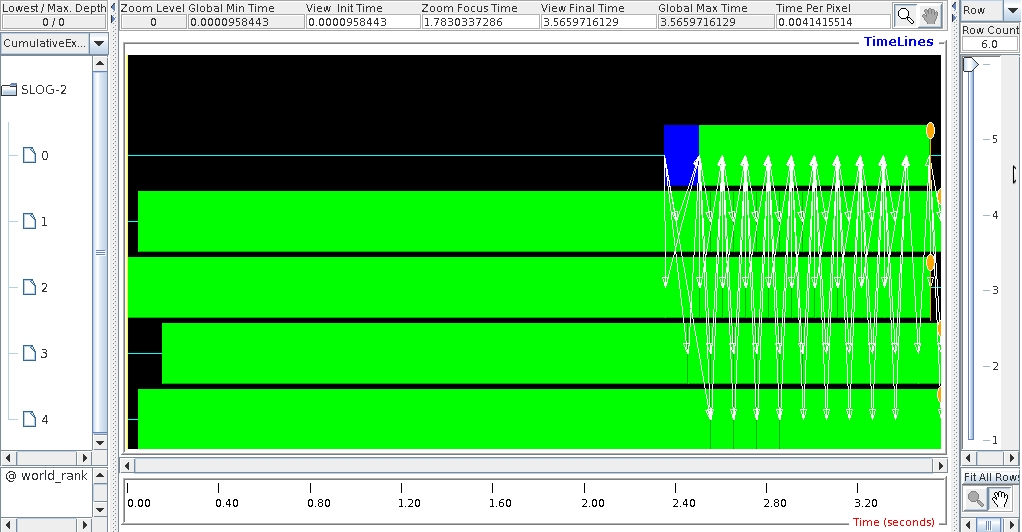
\includegraphics[width=\textwidth]{Immagini_relazione/5_JS5p40.jpg}
\caption{Jumpshot. Utilizzo di 5 processori su 40 sottodomini.}
\label{}
\end{figure}

\newpage
\subsection*{Conclusioni}
Per nostra curiosit\`a, abbiamo concluso l'esercitazione analizzando ancora due situazioni riportate in seguito.
\\
In \emph{Figura \ref{fig:nopartiz}} abbiamo ipotizzato di non poter sfruttare i vantaggi del calcolo parallelo e abbiamo affidato, senza bilanciamento del carico, l'intero dominio ad un unico worker, mentre in \emph{Figura \ref{fig:sottodom}} abbiamo diviso il dominio in tanti sottodomini quanto il numero di slaves. Questi sono i prevedibili risultati:


\begin{figure}[htbp]
\centering
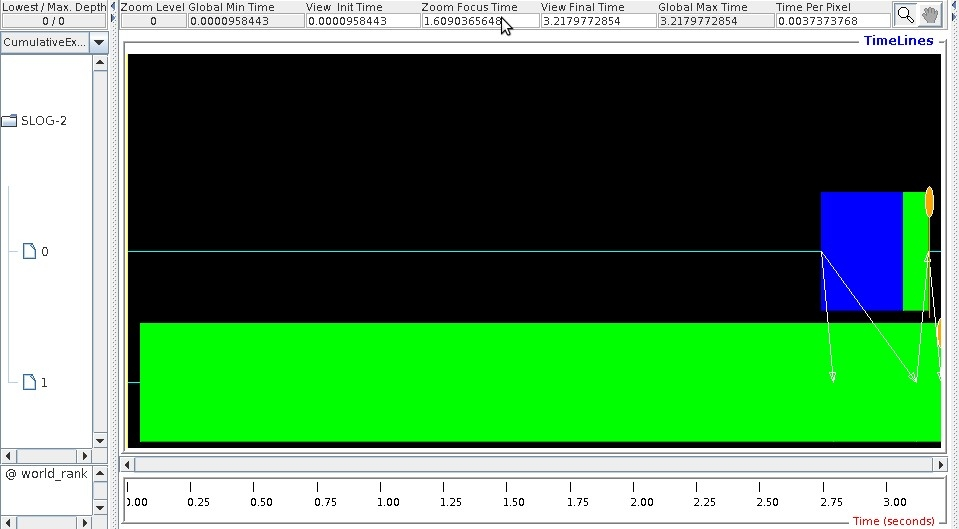
\includegraphics[width=\textwidth]{Immagini_relazione/2pCiascuno1.jpeg}
\caption{Jumpshot. Utilizzo di 2 processori senza partizionare il dominio.}
\label{fig:nopartiz}
\end{figure}

\begin{figure}[htbp]
\centering
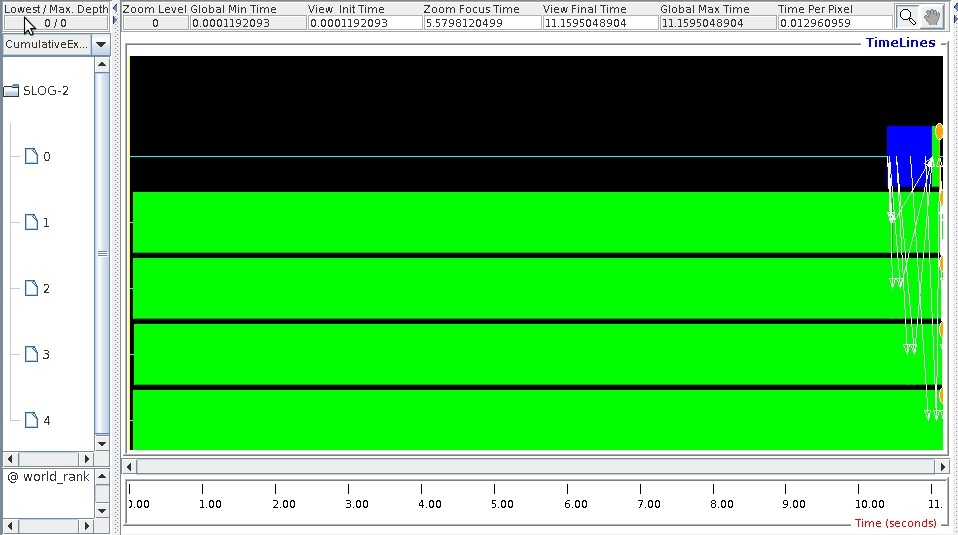
\includegraphics[width=\textwidth]{Immagini_relazione/5pCiascuno4.jpeg}
\caption{Jumpshot. Utilizzo di 5 processori su 4 sottodomini.}
\label{fig:sottodom}
\end{figure}


%\end{document}
